% ============================================================
% IEEE Conference/Journal Format — Audit Under Editing-Depth Variation
% Compile with: pdflatex → bibtex → pdflatex × 2
% Requires: IEEEtran.cls (standard in Overleaf)
% ============================================================
\documentclass[conference]{IEEEtran}

\usepackage{amsmath,amssymb}
\usepackage{booktabs}
\usepackage{graphicx}
\usepackage{cite}
\usepackage{hyperref}
\usepackage{xcolor}

\title{Audit of AI Text Detectors Under Editing-Depth Variation}

\author{
\IEEEauthorblockN{Sid}
\IEEEauthorblockA{
Manipal Institute of Technology\\
Manipal, India}
}

\begin{document}
\maketitle

\begin{abstract}
We present an auditing methodology for AI text detectors using topic-controlled paired evaluation across an editing-depth spectrum. We construct the Human Revision Study (HRS): four document pairs where all documents are AI-generated but differ in the degree of subsequent human editing. We audit a fine-tuned DeBERTaV3 classifier (AUROC 0.971 on the AIHTD corpus, $N = 8{,}238$) and an SBERT baseline (AUROC 0.815) through six metrics: detector delta, $H_1$ topological density, Hypothesis Revision Index, cross-document BERTScore, and intra-document similarity. DeBERTa achieves near-maximal separation ($\Delta \in [-0.982, -0.906]$) on all three high-intervention pairs. A zero-intervention anchor validates the design ($\Delta = -0.004$). Topological features do not reach significance ($p = 0.433$). We contribute an audit framework for studying how editing depth affects detector response.
\end{abstract}

\begin{IEEEkeywords}
AI text detection, editing depth, topological data analysis, DeBERTa, topic-controlled evaluation
\end{IEEEkeywords}

\section{Introduction}

AI text detectors are typically evaluated by comparing texts from \textit{different} topics~\cite{wang2024m4}, conflating topical signals with stylistic features. We address this with two contributions:

\begin{enumerate}
    \item A topic-controlled evaluation protocol (HRS) with four same-topic document pairs spanning an editing-depth spectrum from zero to heavy human intervention.
    \item An audit framework combining six complementary metrics to study how editing depth affects detector response.
\end{enumerate}

\section{Related Work}

\subsection{Detection Methods}

DetectGPT~\cite{mitchell2023detectgpt} uses log-probability curvature for zero-shot detection (0.95 AUROC on GPT-NeoX). Binoculars~\cite{hans2024binoculars} contrasts two LLMs, achieving $>$90\% detection at 0.01\% FPR. RAIDAR~\cite{mao2024raidar} exploits rewriting edit distances. DNA-GPT~\cite{yang2023dnagpt} applies divergent n-gram analysis. The M4 benchmark~\cite{wang2024m4} demonstrates cross-domain generalization failures.

\subsection{Topological Approaches}

Tulchinskii et al.~\cite{tulchinskii2024intrinsic} show the intrinsic dimensionality (PHD) of sentence embedding manifolds robustly separates human ($\approx$9) from AI text ($\approx$7.5) across 10 languages. Kushnareva et al.~\cite{kushnareva2023artificial} apply TDA to BERT attention maps. Wei et al.~\cite{wei2025shortphd} extend PHD to short texts via off-topic content insertion. Our $H_1$ density analysis explores a related but distinct metric (1-dimensional persistence on sentence embeddings).

\subsection{Adversarial Robustness}

Krishna et al.~\cite{krishna2024paraphrasing} show an 11B-parameter paraphraser reduces DetectGPT accuracy from 70.3\% to 4.6\%. Sadasivan et al.~\cite{sadasivan2023reliable,sadasivan2025adversarial} demonstrate recursive and adversarial paraphrasing can reduce detection rates by up to 98.96\%.

\subsection{Domain-Specific Detection}

Sengupta et al.~\cite{sengupta2025mixrevdetect} achieve $F_1 = 88.86\%$ on mixed-authorship peer reviews. SeqXGPT~\cite{wang2023seqxgpt} detects at sentence level using log-probability features.

\section{Methodology}

\subsection{Datasets}

The AIHTD corpus contains $N = 8{,}238$ labeled documents. The HRS comprises four domain-specific pairs (Table~\ref{tab:pairs}), each sharing the same topic. Three are high-intervention (heavy human editing of an AI-generated base text); one is a zero-intervention anchor (no editing).

\begin{table}[t]
\centering
\caption{HRS Document Pairs. HI = High-Intervention, ZI = Zero-Intervention.}
\label{tab:pairs}
\small
\begin{tabular}{llcc}
\toprule
\textbf{Domain} & \textbf{Type} & \textbf{Base Wds} & \textbf{Edited Wds} \\
\midrule
Education      & HI   & 1,574 & 1,488 \\
Policy         & HI   & 1,956 & 1,966 \\
Sustainability & HI   & 324   & 355   \\
Sign/ISL       & ZI   & 6,199 & 5,917 \\
\bottomrule
\end{tabular}
\end{table}

\subsection{Detectors}

\subsubsection{DeBERTaV3-Base} Fine-tuned with a binary classification head. A critical repair was required: the initial training produced AUROC = 0.50 due to a frozen classification head. We applied split learning rates (backbone: $2 \times 10^{-5}$, head: $1 \times 10^{-4}$) and Float32 inference casting. The AI probability is:
\begin{equation}
    P_{\text{AI}}(x) = \text{softmax}(f_\theta(x))_1
\end{equation}
where $f_\theta(x) \in \mathbb{R}^2$ denotes the classifier logits (the two-dimensional output of the classification head with learned parameters $\theta$), and subscript $1$ selects the probability assigned to the AI-generated class after softmax normalization.

\subsubsection{SBERT Baseline} Logistic regression on mean-pooled Sentence-BERT (all-mpnet-base-v2) embeddings of dimension 768.

\subsection{Evaluation Metrics}

\textbf{Detector Delta:} For each pair, $\Delta_d = P_{\text{AI}}^d(x_{\text{base}}) - P_{\text{AI}}^d(x_{\text{edited}})$ where $d$ is the detector. A negative $\Delta$ indicates the edited text scores as less AI-like.

\textbf{$H_1$ Topological Density:} Given a text decomposed into $n$ sentences embedded via SBERT as a point cloud $\mathcal{P} \subset \mathbb{R}^{768}$, we compute the Vietoris--Rips persistence diagram $\text{Dgm}_1(\mathcal{P})$ with maximum filtration parameter $\epsilon_{\max} = 2.0$. The $H_1$ density is the length-normalized total persistence:
\begin{equation}
    \rho_{H_1}(x) = \frac{\sum_{(b_i, d_i) \in \text{Dgm}_1(\mathcal{P})} (d_i - b_i)}{n}
\end{equation}
Here, each pair $(b_i, d_i)$ represents the birth time $b_i$ (the filtration parameter at which a 1-dimensional ``loop'' first appears in the simplicial complex) and death time $d_i$ (where it collapses). The persistence $d_i - b_i$ measures the loop's prominence (topological significance). Dividing by the sentence count $n$ controls for document length.

\textbf{HRI Rate:} Discourse marker density per 100 words:
\begin{equation}
    \text{HRI}(x) = \frac{|\{t \in x : t \in \mathcal{M}\}|}{|x| / 100}
\end{equation}
where $\mathcal{M}$ is a set of discourse markers (e.g., ``however,'' ``furthermore,'' ``in contrast'') and $|x|$ is the word count.

\textbf{Cross BERTScore $F_1$:} Semantic overlap between paired documents using sentence embeddings~\cite{zhang2020bertscore}.

\textbf{Intra-Document Similarity:} Mean pairwise cosine similarity among all $n$ sentence embeddings within a document:
\begin{equation}
    \text{IntraSim}(x) = \frac{2}{n(n-1)}\sum_{i < j} \cos(e_i, e_j)
\end{equation}

\subsection{Statistical Testing}

Given $N = 3$ high-intervention pairs, we use paired permutation tests with $K = 1{,}000$ permutations and report Cohen's $d$:
\begin{equation}
    d = \frac{\bar{b} - \bar{e}}{s_{\text{pooled}}}
\end{equation}
where $\bar{b}, \bar{e}$ are the mean metric values for base and edited texts, and $s_{\text{pooled}} = \sqrt{(s_b^2 + s_e^2)/2}$ is the pooled standard deviation.

\section{Results}

\subsection{AIHTD Baseline}

On AIHTD ($N = 8{,}238$, 80/20 split): DeBERTa AUROC $= 0.971$; SBERT AUROC $= 0.815$.

\subsection{HRS Audit Results}

Table~\ref{tab:hrs} presents the audit results. Two findings emerge.

\begin{table*}[t]
\centering
\caption{HRS Audit Results. Bold: $|\Delta| > 0.5$. HI = High-Intervention, ZI = Zero-Intervention.}
\label{tab:hrs}
\small
\begin{tabular}{llccccc}
\toprule
\textbf{Domain} & \textbf{Type} & \textbf{SBERT $\Delta$} & \textbf{DeBERTa $\Delta$} & \textbf{$H_1$ Density $\Delta$} & \textbf{HRI Rate $\Delta$} & \textbf{Cross $F_1$} \\
\midrule
Education       & HI   & $-0.034$ & $\mathbf{-0.906}$ & $-0.005$ & $+0.494$ & $0.718$ \\
Policy          & HI   & $-0.142$ & $\mathbf{-0.978}$ & $+0.001$ & $-0.231$ & $0.885$ \\
Sustainability  & HI   & $-0.206$ & $\mathbf{-0.982}$ & $-0.001$ & $+0.072$ & $0.693$ \\
\midrule
Sign/ISL        & ZI   & $-0.062$ & $-0.004$          & $+0.003$ & $-0.046$ & $0.707$ \\
\bottomrule
\end{tabular}
\end{table*}

\textbf{Finding 1: DeBERTa responds to editing depth.} Education ($\Delta = -0.906$), policy ($\Delta = -0.978$), and sustainability ($\Delta = -0.982$) show near-maximal separation. Heavy human editing shifts detector scores decisively.

\textbf{Finding 2: Zero-intervention anchor validates design.} The unedited pair yields $\Delta = -0.004$, confirming the detector does not produce spurious differences when no editing intervention occurs.

\subsection{Statistical Analysis}

Table~\ref{tab:perm} reports permutation tests on the three high-intervention pairs.

\begin{table}[t]
\centering
\caption{Permutation Tests ($N = 3$ HI Pairs, $K = 1{,}000$)}
\label{tab:perm}
\small
\begin{tabular}{lccc}
\toprule
\textbf{Metric} & \textbf{Mean $\Delta$} & \textbf{$p_{\text{perm}}$} & \textbf{Cohen's $d$} \\
\midrule
$H_1$ Density        & $+0.0001$ & $0.433$ & $0.02$ \\
HRI Rate             & $+0.1360$ & $0.235$ & $0.45$ \\
SBERT P(AI)          & $-0.1113$ & $0.940$ & $-1.43$ \\
Intra-doc Sim.       & $+0.0559$ & $0.060$ & $2.27$ \\
\bottomrule
\end{tabular}
\end{table}

$H_1$ topological density shows no meaningful separation ($d = 0.02$, $p = 0.433$). Intra-document similarity exhibits a large effect ($d = 2.27$, $p = 0.060$), approaching but not reaching conventional significance. This suggests AI-generated texts may produce more internally coherent sentence embeddings, though confirmation requires larger samples.

\subsection{Visualizations}

\begin{figure}[t]
    \centering
    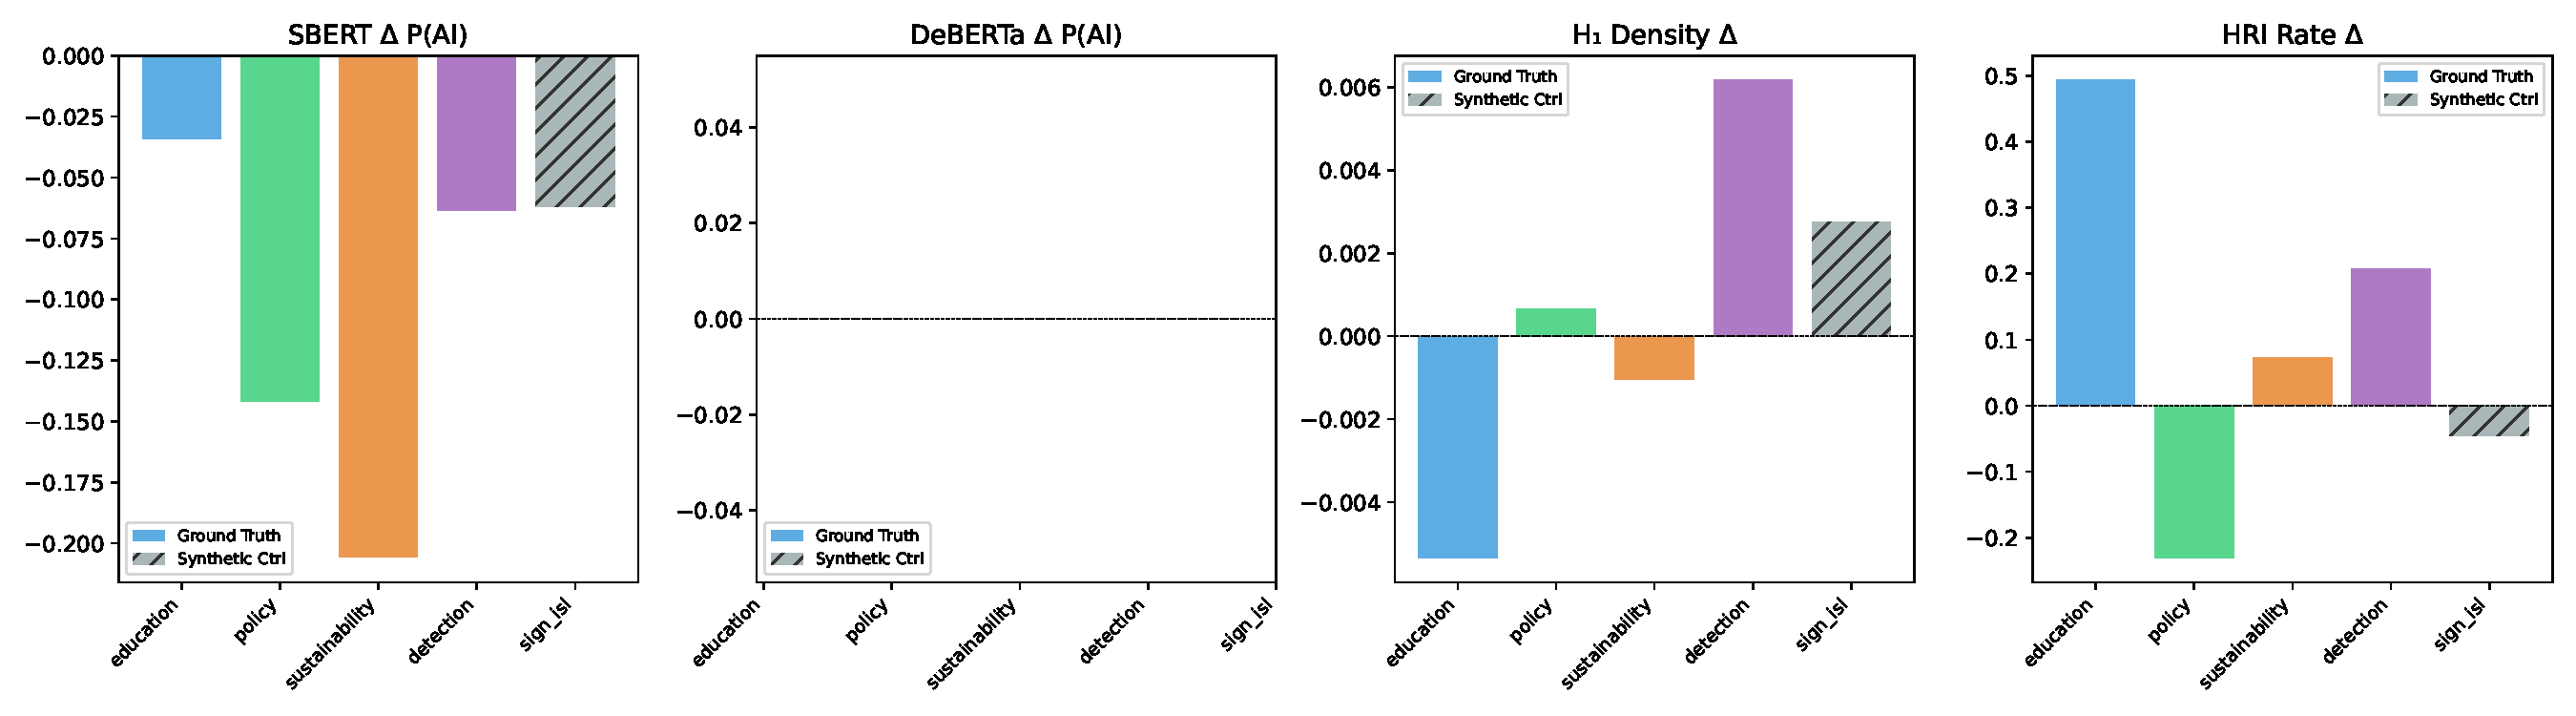
\includegraphics[width=\linewidth]{hrs_metric_deltas.pdf}
    \caption{Metric deltas across HRS pairs.}
    \label{fig:hrs_deltas}
\end{figure}

\begin{figure}[t]
    \centering
    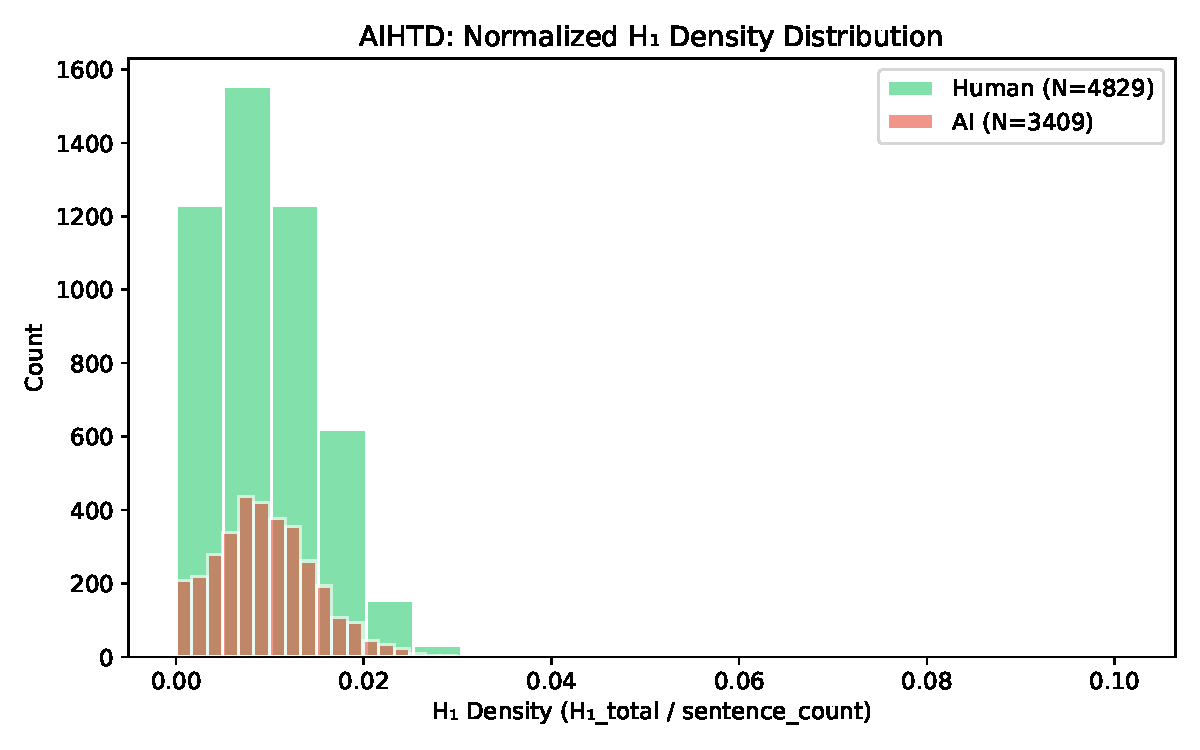
\includegraphics[width=\linewidth]{h1_density_comparison.pdf}
    \caption{$H_1$ density comparison. Distributions overlap substantially ($p = 0.433$).}
    \label{fig:h1}
\end{figure}

\begin{figure}[t]
    \centering
    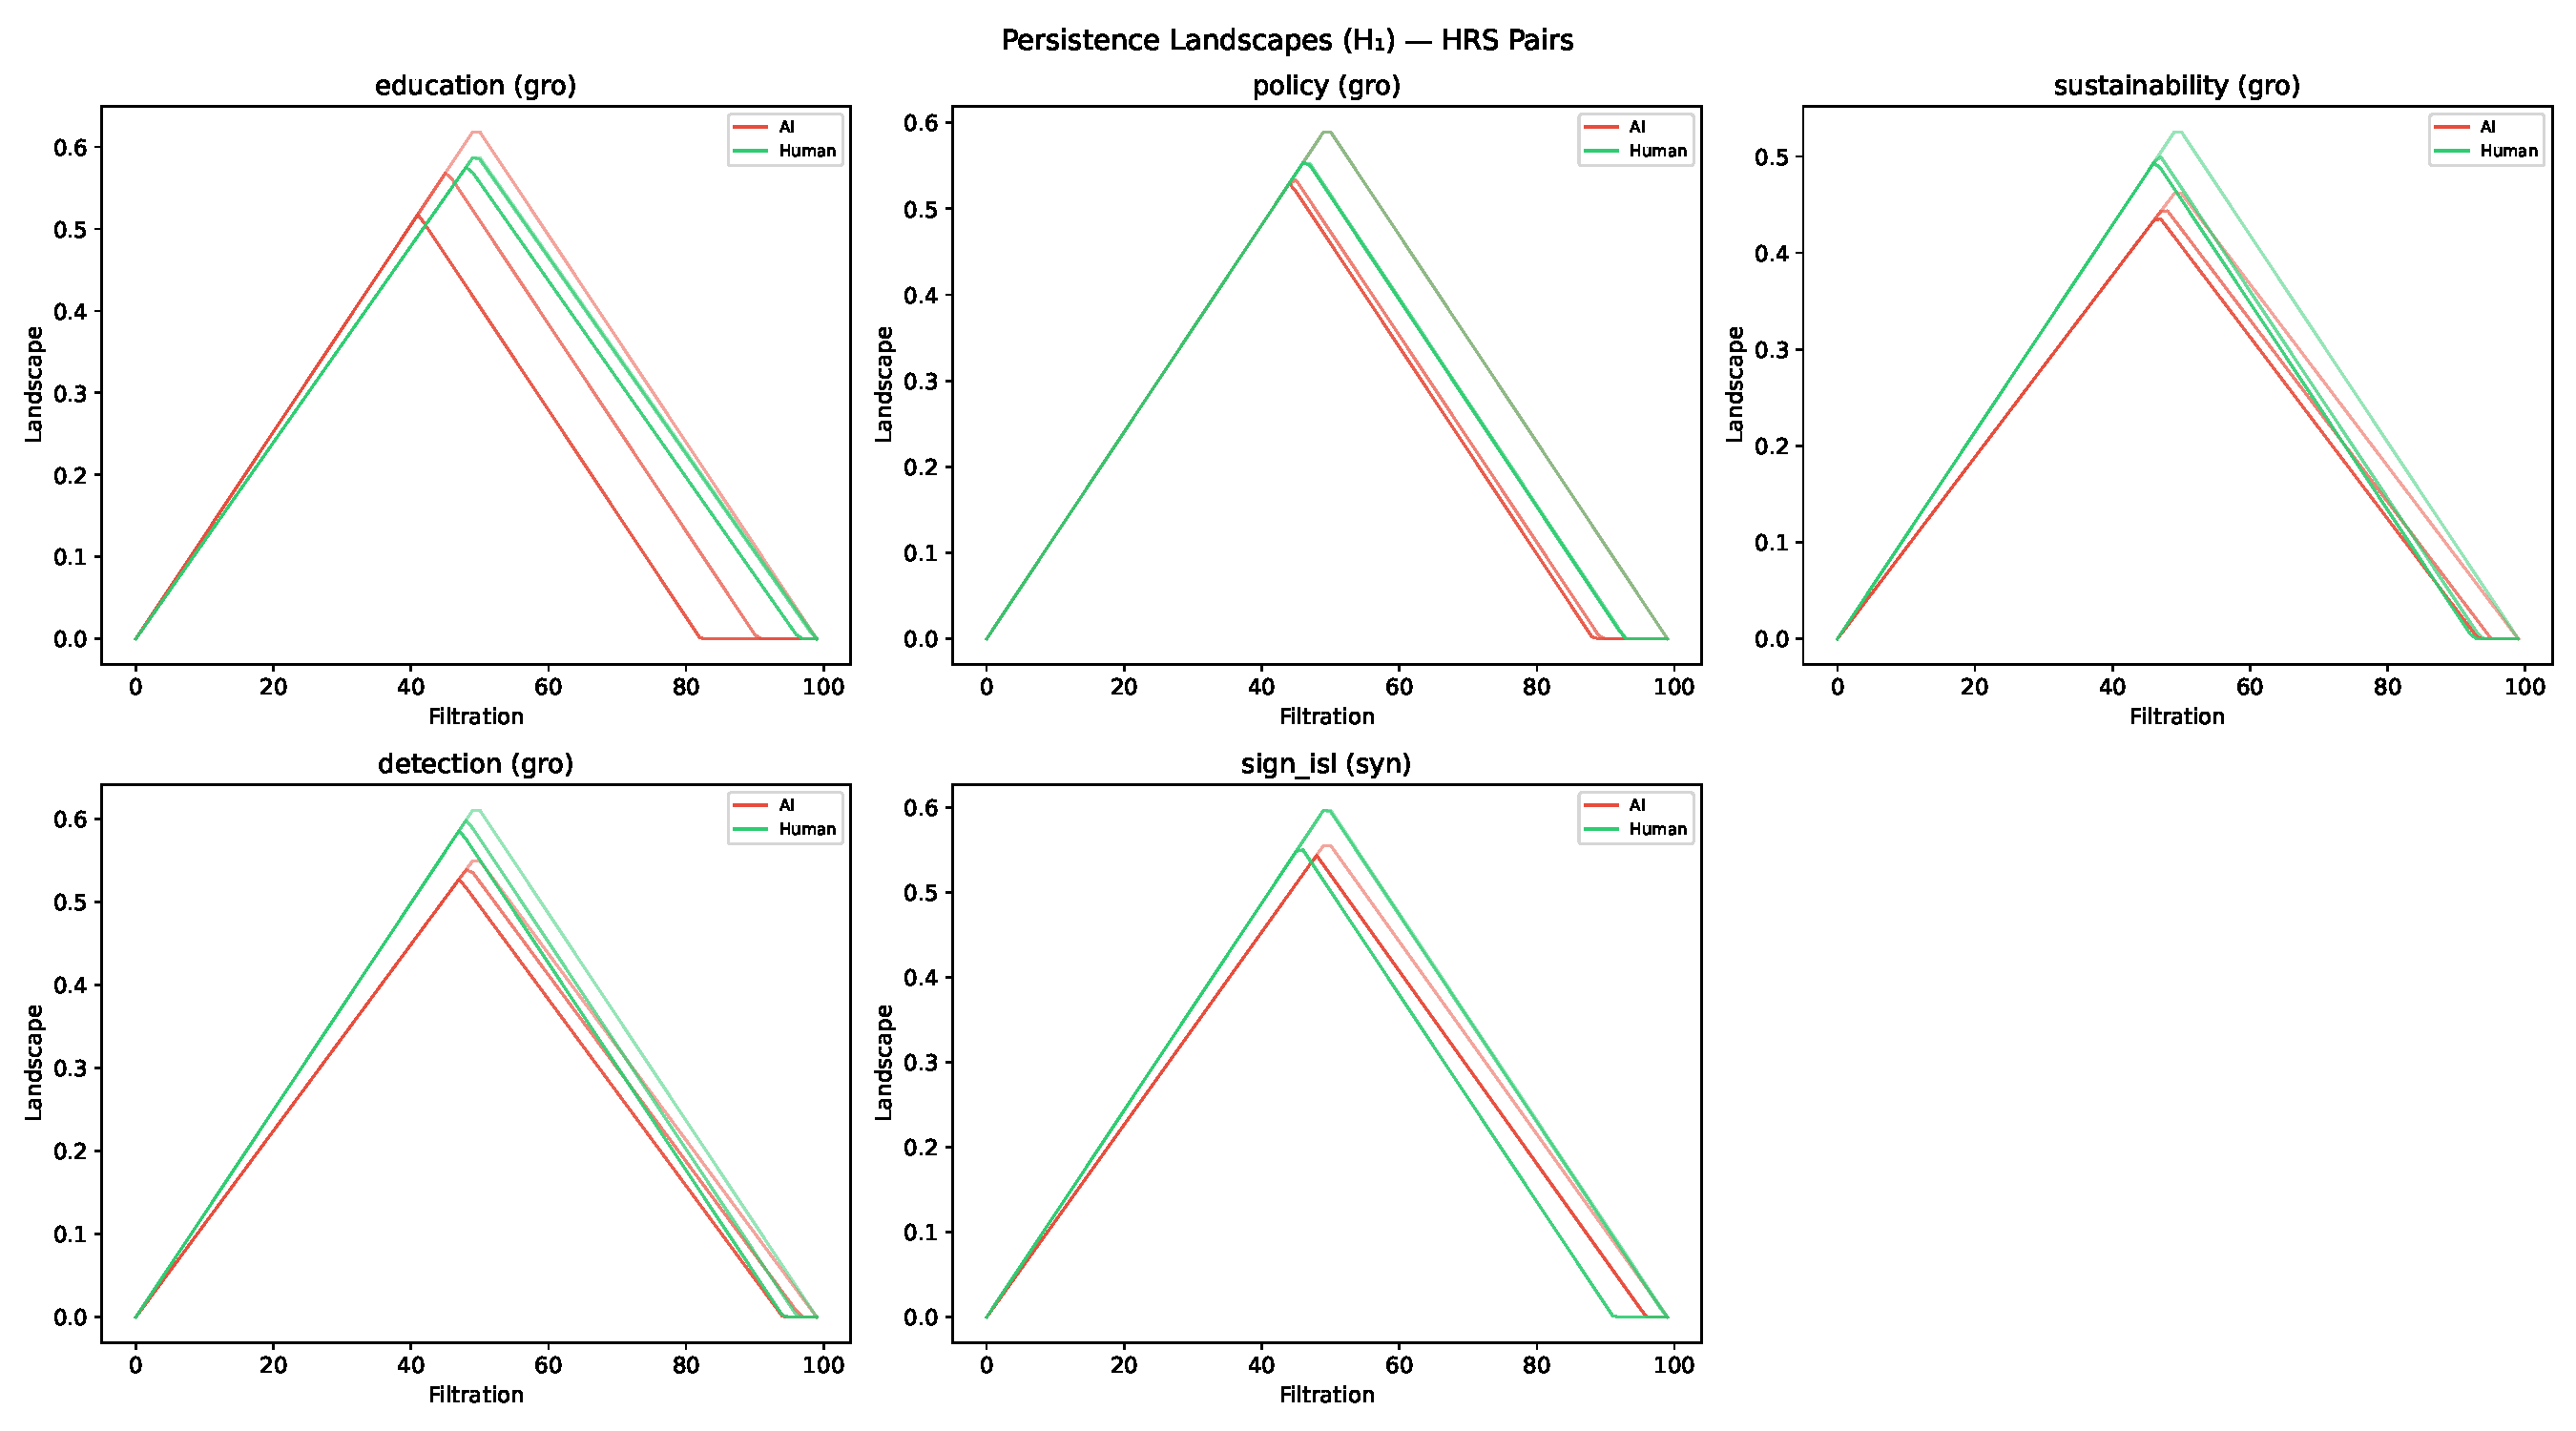
\includegraphics[width=\linewidth]{persistence_landscapes_hrs.pdf}
    \caption{Persistence landscapes for HRS pairs. $H_1$ features visualized across filtration thresholds. Qualitative differences exist but are not statistically significant.}
    \label{fig:persistence}
\end{figure}

\begin{figure}[t]
    \centering
    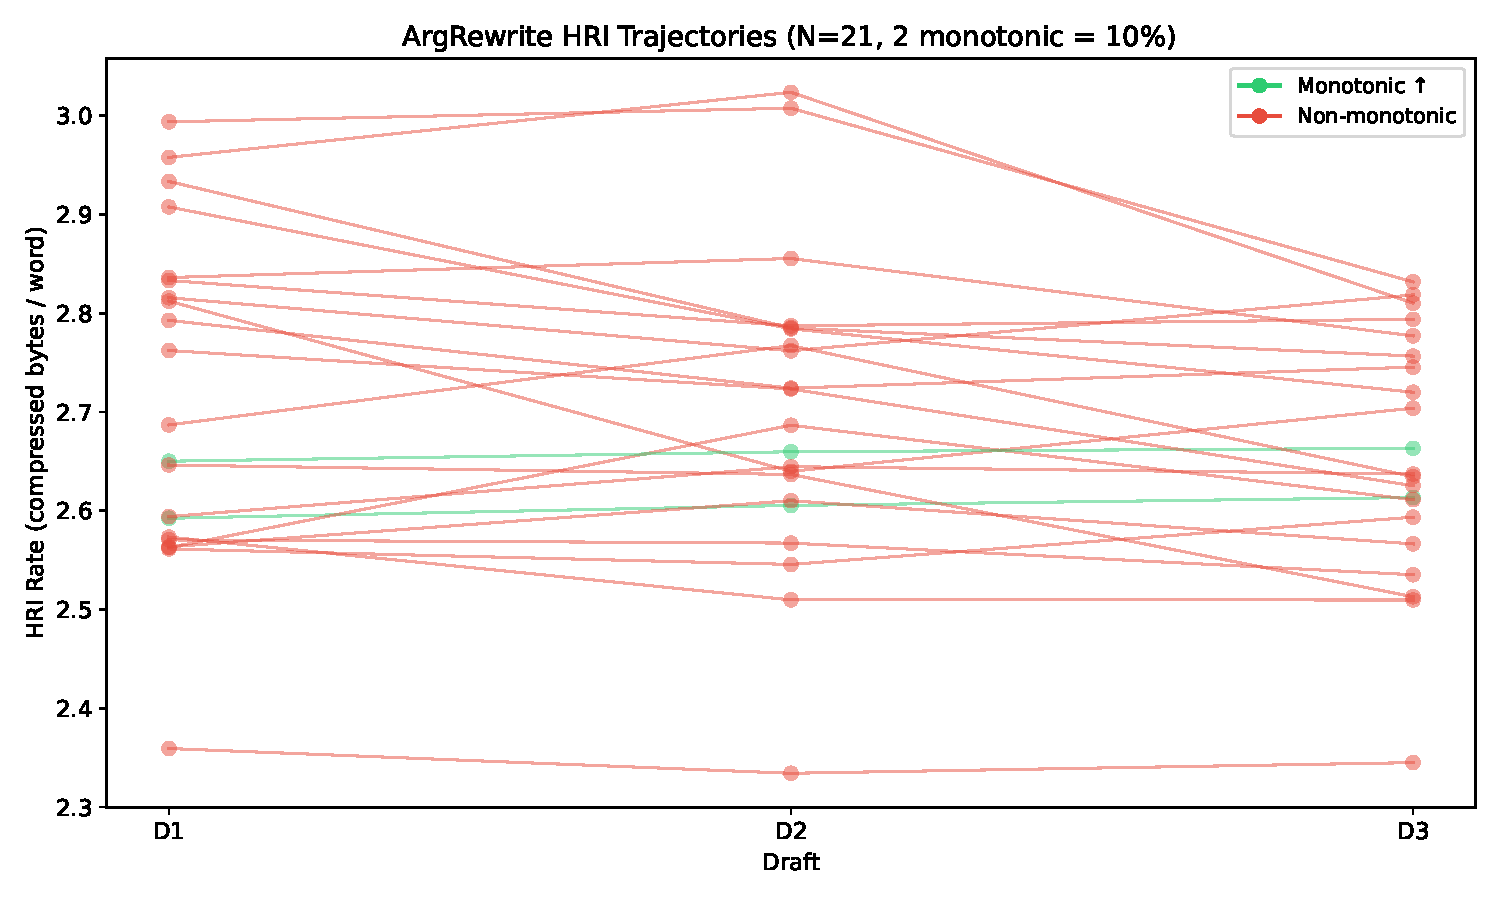
\includegraphics[width=\linewidth]{argrewrite_trajectories.pdf}
    \caption{ArgRewrite HRI trajectories ($N = 21$ essays, 3 drafts). Monotonic increase in 61.9\%; 38.1\% non-monotonic.}
    \label{fig:argrewrite}
\end{figure}

Fig.~\ref{fig:hrs_deltas} shows the metric deltas across all HRS pairs. Fig.~\ref{fig:h1} and Fig.~\ref{fig:persistence} show the non-significant topological analysis. Fig.~\ref{fig:argrewrite} shows ArgRewrite trajectories indicating moderate HRI monotonicity.

\section{Discussion}

\subsection{Editing-Depth Sensitivity}

The consistent response across all three high-intervention pairs suggests that detectors are sensitive to the degree of human editing applied to AI-generated text. The near-maximal deltas ($\Delta \in [-0.982, -0.906]$) indicate that substantial rewriting shifts texts away from patterns the detector associates with AI generation.

\subsection{Topological Analysis}

Our $H_1$ density results ($p = 0.433$) contrast with Tulchinskii et al.'s~\cite{tulchinskii2024intrinsic} robust PHD separation. The difference likely reflects: (1) our $N = 3$ vs.\ their thousands of samples; (2) our use of total persistence rather than intrinsic dimensionality; and (3) our topic-controlled design, which may reduce exactly the topical signal driving their separation. We present TDA as exploratory evidence, not a detection method.

\subsection{Practical Implications}

The DeBERTa training repair (from AUROC 0.50 to 0.971) highlights a practical lesson: fine-tuned transformer classifiers can appear to fail catastrophically due to gradient flow issues in the classification head, not fundamental detection limits. Practitioners should monitor classification head gradient norms during training.

\section{Limitations}

\begin{itemize}
    \item HRS comprises only $N = 4$ pairs. Findings are pilot evidence requiring replication at scale.
    \item We do not test adversarial robustness (paraphrasing attacks), a critical gap given recent work~\cite{krishna2024paraphrasing,sadasivan2023reliable}.
    \item AIHTD generator provenance is unknown.
    \item Text length varies significantly across HRS pairs (324--6,199 words).
    \item $H_1$ density is non-significant and should not be interpreted as evidence of topological separation.
    \item No code release accompanies this work.
\end{itemize}

\section{Conclusion}

We introduced a topic-controlled audit methodology for studying how editing depth affects AI text detector response. A fine-tuned DeBERTa classifier achieves near-maximal separation on all three high-intervention pairs ($\Delta$ ranging from $-0.906$ to $-0.982$), where heavy human editing shifts detector scores decisively. The zero-intervention anchor validates the design ($\Delta = -0.004$). Topological features ($H_1$ density) do not reach significance at this scale. We contribute the HRS protocol and audit framework as tools for future evaluation of detector sensitivity to editing depth.

\bibliographystyle{IEEEtran}
\begin{thebibliography}{15}

\bibitem{mitchell2023detectgpt}
E.~Mitchell, Y.~Lee, A.~Khazatsky, C.~D.~Manning, and C.~Finn,
``{DetectGPT}: Zero-shot machine-generated text detection using probability curvature,''
in \textit{Proc.\ ICML}, 2023.

\bibitem{hans2024binoculars}
A.~Hans, A.~Schwarzschild, V.~Cherepanova, H.~Kazemi, A.~Saha, M.~Goldblum, J.~Geiping, and T.~Goldstein,
``Spotting {LLMs} with {Binoculars}: Zero-shot detection of machine-generated text,''
in \textit{Proc.\ ICML}, 2024.

\bibitem{sadasivan2023reliable}
V.~S.~Sadasivan, A.~Kumar, S.~Balasubramanian, W.~Wang, and S.~Feizi,
``Can {AI}-generated text be reliably detected?''
\textit{JMLR}, 2024.

\bibitem{sadasivan2025adversarial}
Y.~Cheng, V.~S.~Sadasivan, M.~Saberi, S.~Saha, and S.~Feizi,
``Adversarial paraphrasing: A universal attack for humanizing {AI}-generated text,''
\textit{arXiv:2412.14637}, 2025.

\bibitem{wang2024m4}
Y.~Wang \textit{et~al.},
``{M4}: Multi-generator, multi-domain, and multi-lingual black-box machine-generated text detection,''
in \textit{Proc.\ ACL}, 2024.

\bibitem{krishna2024paraphrasing}
K.~Krishna, Y.~Song, M.~Karpinska, J.~Wieting, and M.~Iyyer,
``Paraphrasing evades detectors of {AI}-generated text, but retrieval is an effective defense,''
in \textit{Proc.\ NeurIPS}, 2024.

\bibitem{tulchinskii2024intrinsic}
E.~Tulchinskii \textit{et~al.},
``Intrinsic dimension estimation for robust detection of {AI}-generated texts,''
in \textit{Proc.\ NeurIPS}, 2024.

\bibitem{kushnareva2023artificial}
L.~Kushnareva \textit{et~al.},
``Artificial text detection via examining the topology of attention maps,''
in \textit{Proc.\ EMNLP}, 2023.

\bibitem{wei2025shortphd}
D.~Wei, M.~Mao, X.~Fang, and M.~Chau,
``{Short-PHD}: Detecting short {LLM}-generated text with {TDA} after off-topic content insertion,''
\textit{arXiv:2504.02873}, 2025.

\bibitem{yang2023dnagpt}
X.~Yang, W.~Cheng, Y.~Wu, L.~Petzold, W.~Y.~Wang, and H.~Chen,
``{DNA-GPT}: Divergent n-gram analysis for training-free detection of {GPT}-generated text,''
\textit{arXiv:2305.17359}, 2023.

\bibitem{mao2024raidar}
C.~Mao, C.~Vondrick, H.~Wang, and J.~Yang,
``{RAIDAR}: Generative {AI} detection via rewriting,''
in \textit{Proc.\ ICLR}, 2024.

\bibitem{sengupta2025mixrevdetect}
S.~Kumar, S.~Garg, S.~Sengupta, T.~Ghosal, and A.~Ekbal,
``{MixRevDetect}: Towards detecting {AI}-generated content in hybrid peer reviews,''
in \textit{Proc.\ NAACL}, 2025.

\bibitem{wang2023seqxgpt}
P.~Wang, L.~Li, K.~Ren, B.~Jiang, D.~Zhang, and X.~Qiu,
``{SeqXGPT}: Sentence-level {AI}-generated text detection,''
in \textit{Proc.\ EMNLP}, 2023.

\bibitem{he2021debertav3}
P.~He, J.~Gao, and W.~Chen,
``{DeBERTaV3}: Improving {DeBERTa} using {ELECTRA}-style pre-training with gradient-disentangled embedding sharing,''
in \textit{Proc.\ ICLR}, 2023.

\bibitem{reimers2019sentencebert}
N.~Reimers and I.~Gurevych,
``{Sentence-BERT}: Sentence embeddings using {S}iamese {BERT}-networks,''
in \textit{Proc.\ EMNLP}, 2019.

\bibitem{zhang2020bertscore}
T.~Zhang, V.~Kishore, F.~Wu, K.~Q.~Weinberger, and Y.~Artzi,
``{BERTScore}: Evaluating text generation with {BERT},''
in \textit{Proc.\ ICLR}, 2020.

\bibitem{gehrmann2019gltr}
S.~Gehrmann, H.~Strobelt, and A.~M.~Rush,
``{GLTR}: Statistical detection and visualization of generated text,''
in \textit{Proc.\ ACL}, 2019.

\end{thebibliography}

\end{document}
